
\section{Game}

Gra jest wykonana w środowisku Unity. Należy ona do typu tower defense. Plansza gry składa się z tiles będących trójwymiarowymi modelami dzielącymi się na dwie kategorie: ziemia i droga. Jest jeden tile typu ziemia i pięć tiles typu droga (fig.~\ref{Fig:tiles}).

\begin{figure}
\begin{tikzpicture}
\node[anchor=center,inner sep=0, label=below:{Ground}] at (-4,3) {
\includegraphics[width=2cm]{images/tileGround.png}};
\node[anchor=center,inner sep=0, label=below:{Water}] at (-4,1) {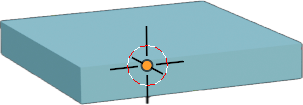
\includegraphics[width=2cm]{images/tileWater.png}};
\node[anchor=center,inner sep=0,label=below:{Straight}] (tikz) at (-1.5,1) {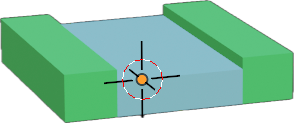
\includegraphics[width=2cm]{images/tileWaterStraight.png}};
\node[anchor=center,inner sep=0,label=below:{Curve}] (tikz) at (1,1) {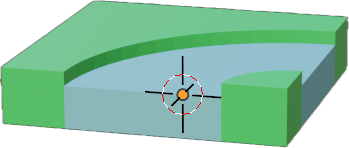
\includegraphics[width=2cm]{images/tileWaterCurve.png}};
\node[anchor=center,inner sep=0,label=below:{Intersection 1}] (tikz) at (3.5,1) {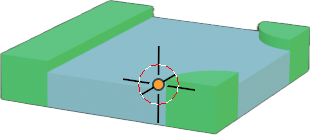
\includegraphics[width=2cm]{images/tileWaterIntersection1.png}};
\node[anchor=center,inner sep=0,label=below:{Intersection 2}] (tikz) at (6,1) {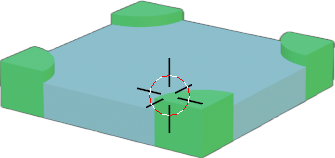
\includegraphics[width=2cm]{images/tileWaterIntersection2.png}};
\end{tikzpicture}

\caption{Modele tiles}
\label{Fig:tiles}
\end{figure}  

Na rysunku~\ref{Fig:changeTiles} pokazano w którym miejscu w interfejsie edytora Unity należy zmienić modele tiles (o ile to będzie istniała taka  potrzeba). Górne zaznaczenie pokazuje miejsce zmiany modelu tile typu ziemia. Dolne zaznaczenie pokazuje miejsce zmiany pierwszego modelu tile typu droga. Pozostałe znajdują się w WaterStraight, WaterCurve itd. Elementy WaterBegin, WaterBeginEnd itp. są kombinacją modeli z rysunku~\ref{Fig:tiles} ze strzałkami. 

\begin{figure}
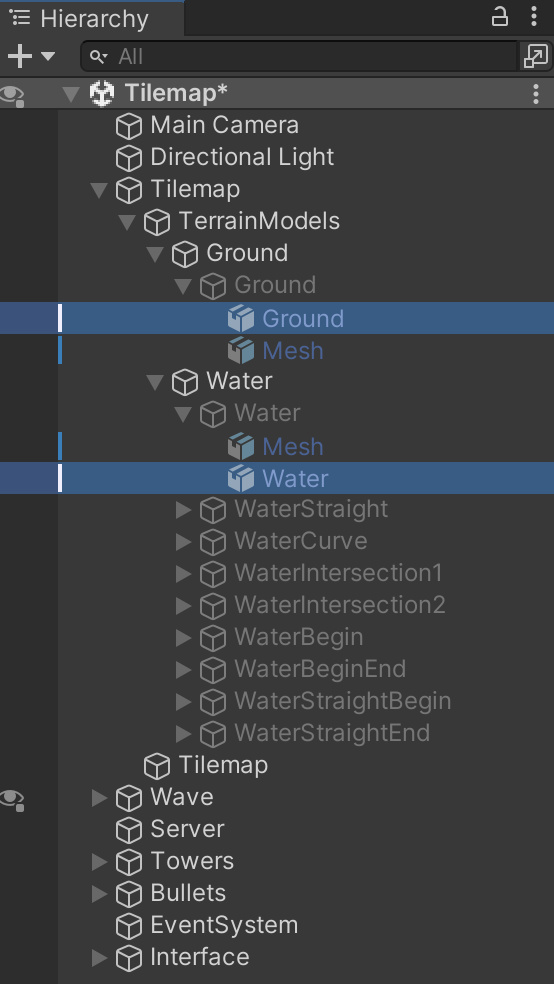
\includegraphics[width=5cm]{images/changeTiles.png}
\caption{Zmiana modeli tiles}
\label{Fig:changeTiles}
\end{figure}  

Na podobnej zasadzie można zmieniać model przeciwników i wież. Miejsce zmian modeli są pokazane na rysunkach~\ref{Fig:changeEnemy} i ~\ref{Fig:changeTower}.

\begin{figure}
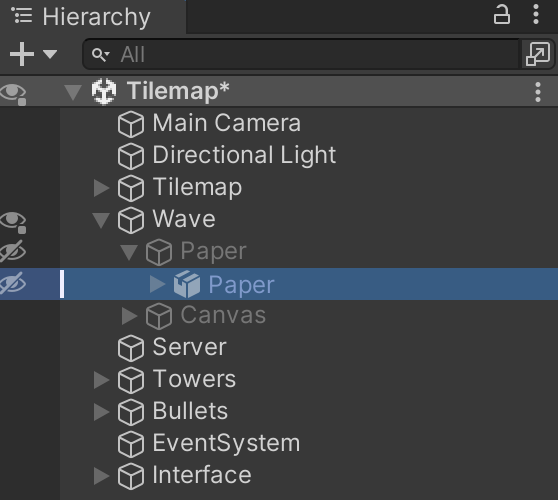
\includegraphics[width=5cm]{images/changeEnemy.png}
\caption{Zmiana modelu przeciwnika}
\label{Fig:changeEnemy}
\end{figure}  


\begin{figure}
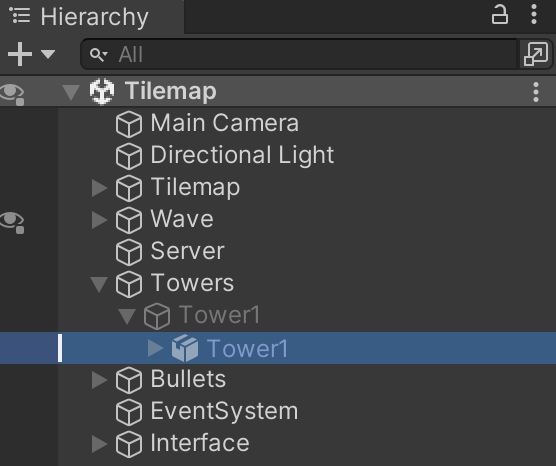
\includegraphics[width=5cm]{images/changeTower.png}
\caption{Zmiana modelu wieży}
\label{Fig:changeTower}
\end{figure}  

Rysunek~\ref{Fig:enemyParameters}  przedstawia miejsce w którym w edytorze Unity można zmienić parametry przeciwników:
\begin{itemize}
\item Speed -- prędkość poruszania się,
\item Start health -- start health,
\item Armour -- wartość odejmowana od zadanych obrażeń (powoduje niewrażliwość na pociski, które mają niższą liczbę zadawanych obrażeń od Armour),
\item Coins -- liczba coins potrzebna do utworzenia przeciwnika,
\item Destroy Coins -- liczba coins jaką otrzymują wieże za zabicie przeciwnika,
\item Coins To End -- liczba coins jaką otrzymują przeciwnicy jeżeli przeciwnik dotrze do punktu końcowego,
\item Count -- liczba dostępnych przeciwników (-1 oznacza niegraniczoną liczbę przeciwników).  
\end{itemize}

\begin{figure}
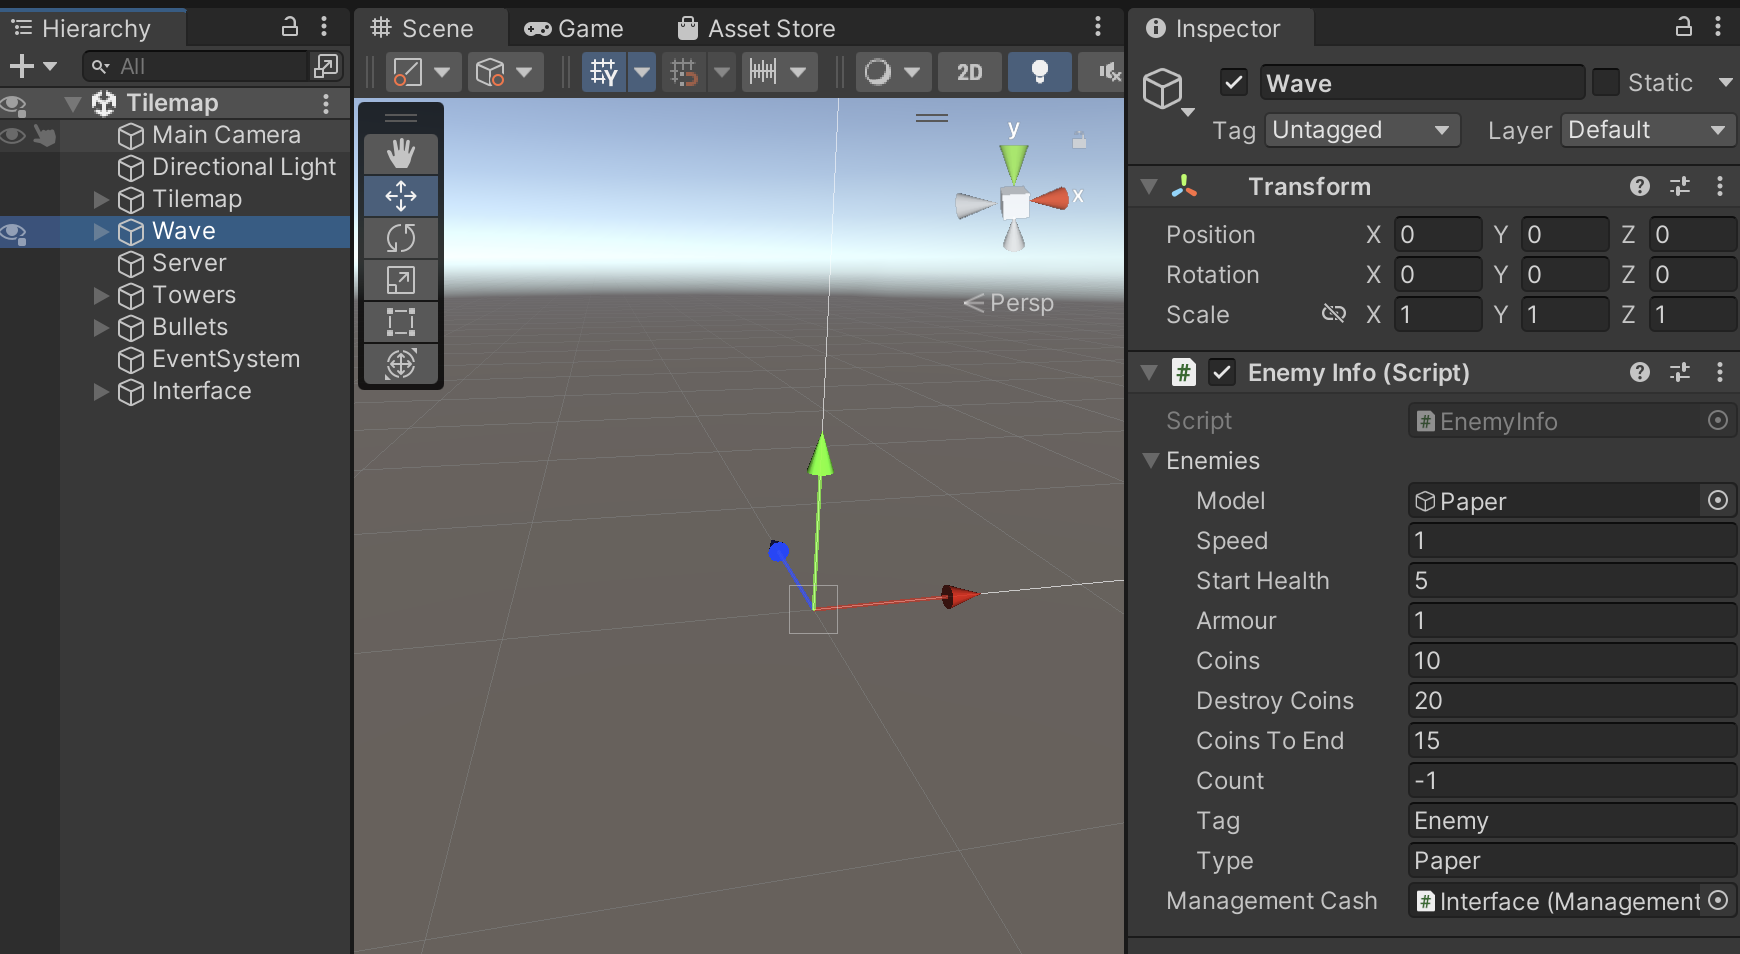
\includegraphics[width=15cm]{images/enemyParameters.png}
\caption{Zmiana parametrów przeciwników}
\label{Fig:enemyParameters}
\end{figure}  

Rysunek~\ref{Fig:towerParameters}  przedstawia miejsce w którym w edytorze Unity można zmienić parametry wież:
\begin{itemize}
\item Speed -- prędkość obrotu,
\item Rate Od Fire -- szybkostrzelność,
\item Bullet Strength -- liczba zadawanych obrażeń,
\item Force -- siła wystrzelenia pocisku przekładająca się na jego zasięg,
\item Coins -- liczba coins potrzebna do utworzenia wieży,
\item Count -- liczba dostępnych wież (-1 oznacza niegraniczoną liczbę wież).  
\end{itemize}

\begin{figure}
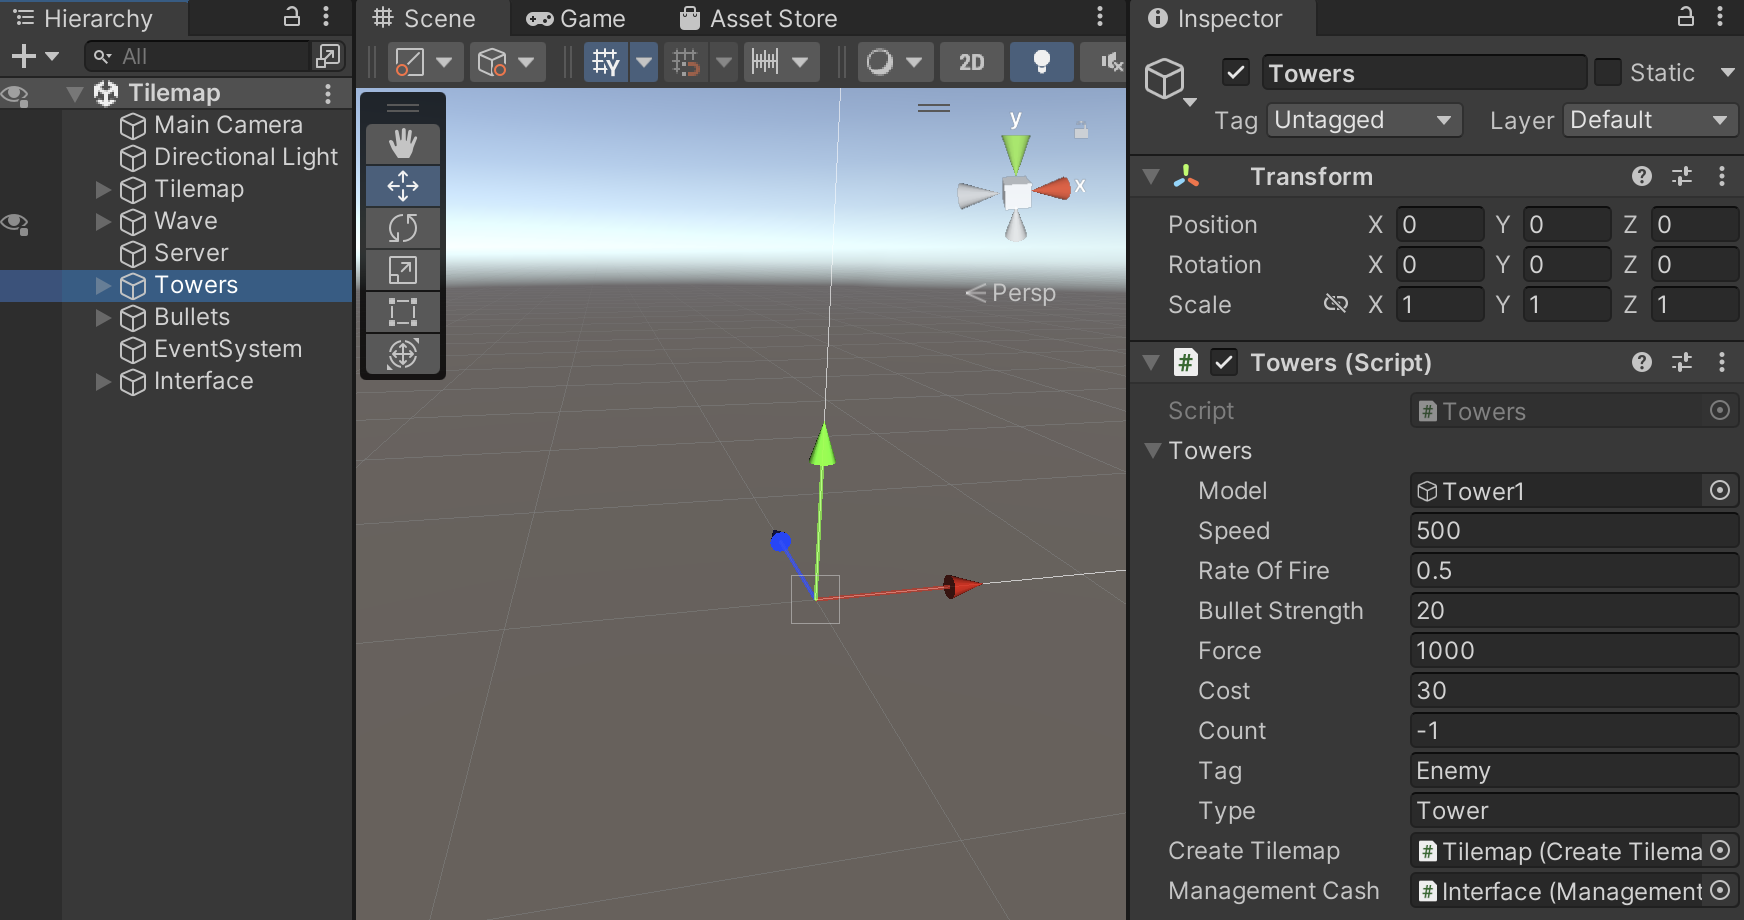
\includegraphics[width=15cm]{images/towerParameters.png}
\caption{Zmiana parametrów wież}
\label{Fig:towerParameters}
\end{figure}  

Rysunek~\ref{Fig:startCoins}  przedstawia miejsce w którym w edytorze Unity można zmienić początkową liczbę coins:
\begin{itemize}
\item Start Coins --  początkowa liczba coins wież; 
\item Start Enemy Coins --  początkowa liczba coins przeciwników. 
\end{itemize}


\begin{figure}
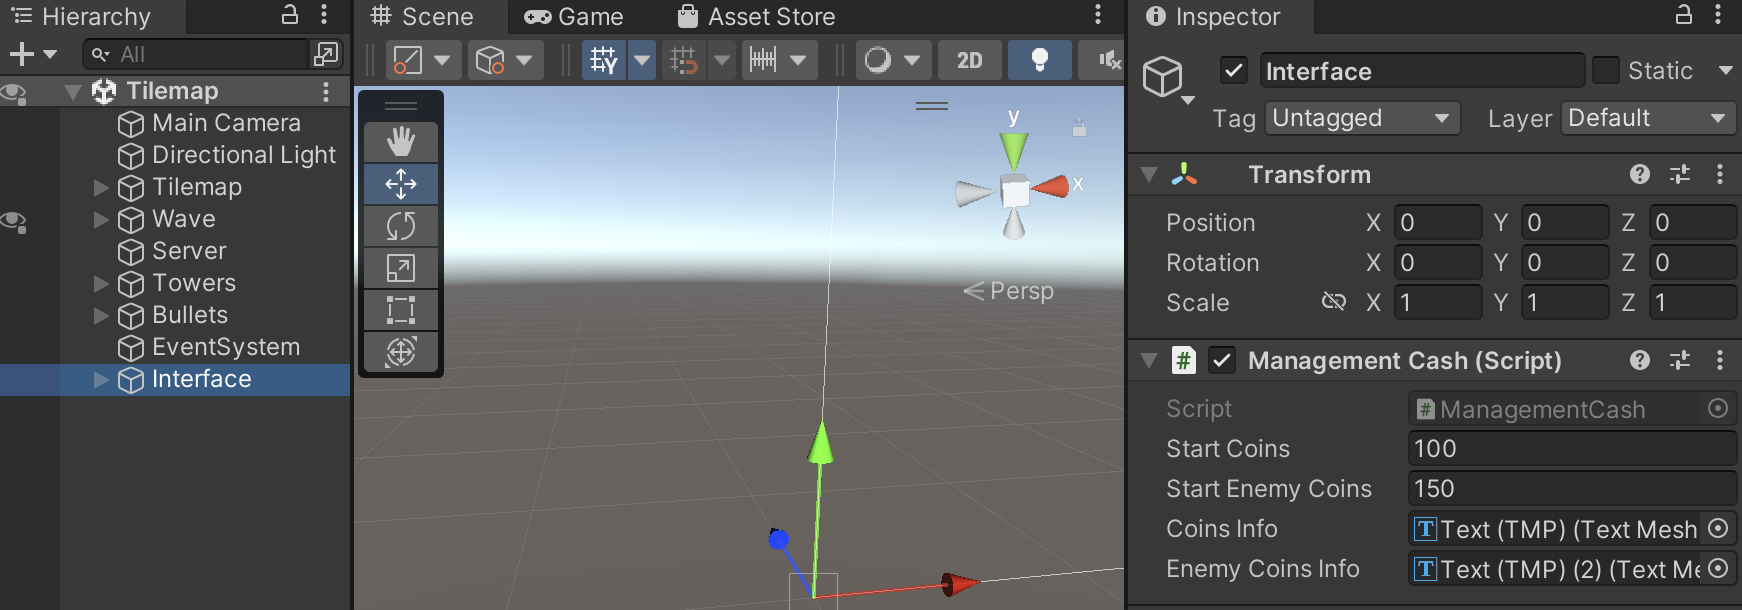
\includegraphics[width=15cm]{images/startCoins}
\caption{Początkowe coins}
\label{Fig:startCoins}
\end{figure} 

Rysunek~\ref{Fig:serverParameters}  przedstawia miejsce w którym w edytorze Unity można zmienić parametry serwera: 
\begin{itemize}
\item IP Adress --  adres ip serwera (127.0.0.1 oznacza, że serwer będzie dostępny tylko dla oprogramowania zainstalowanego na tym samym komputerze co gra); 
\item Port --  port na którym nasłuchuje serwer. 
\end{itemize}

\begin{figure}
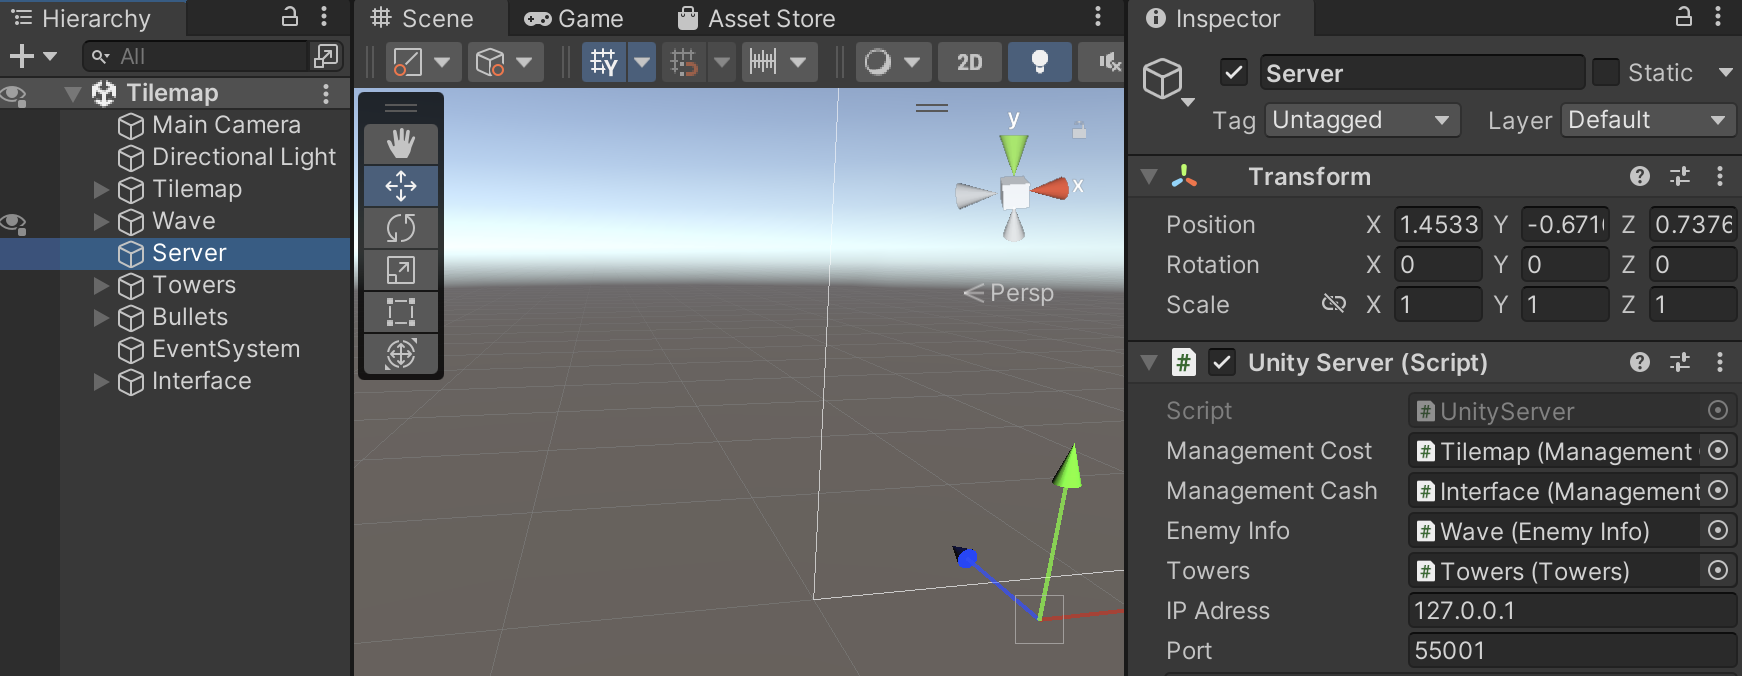
\includegraphics[width=15cm]{images/serverParameters.png}
\caption{Parametry serwera komunikacyjnego}
\label{Fig:serverParameters}
\end{figure} 

Planszę gry stanowi zbiór $n \times m$ tiles mających podstawę kwadratu. $n$ i $m$ to odpowiednio szerokość i wysokość planszy wyrażona w długościach boku kwadratu będącego podstawą tile. Przykładowy XML  definiujący planszę gry:
\lstinputlisting[language=XML]{xml/tilemap.xml}

Po wysłaniu danych, zwracana jest informacja w postaci XML. W przypadku definicji planszy gry zwracane są dane XML z informacją o poprawności (lub nie) informacji przekazanej do serwera:
\lstinputlisting[language=XML]{xml/tilemapResponse.xml}

XML definiujący parametry przeciwników:
\lstinputlisting[language=XML]{xml/enemy.xml}

Po zdefiniowaniu parametrów zwracana jest informacja o poprawności wykonania komendy (analogiczna jak w przypadku tilemap). 

XML definiujący parametry wież:
\lstinputlisting[language=XML]{xml/tower.xml}

Po definiowaniu parametrów zwracana jest informacja o poprawności wykonania komendy (analogiczna jak w przypadku tilemap). 

Utworzenie przeciwnika i wypuszczenie go wybraną ścieżką:
\lstinputlisting[language=XML]{xml/addEnemy.xml}

Po utworzeniu przeciwnika zwracana jest informacja o poprawności wykonania komendy (analogiczna jak w przypadku tilemap). 

XML powodujący dodanie nowej wieży:
\lstinputlisting[language=XML]{xml/addTower.xml}

Po dodaniu nowej wieży zwracana jest informacja o poprawności wykonania komendy (analogiczna jak w przypadku tilemap). 

Żądanie przesłania informacji o ścieżkach:
\lstinputlisting[language=XML]{xml/GetChoiceOfPathData.xml}

Zwracana przez serwer informacja:
\lstinputlisting[language=XML]{xml/GetChoiceOfPathDataResponse.xml}

Żądanie przesłania szczegółowych informacji o stanie gry:
\lstinputlisting[language=XML]{xml/LevelData.xml}

Zwracana przez serwer informacja:
\lstinputlisting[language=XML]{xml/LevelDataResponse.xml}
